\chapter{Evaluation}
\label{ch:Evaluation}
This chapter aims to validate the hypotheses formulated for two distinct studies described in Chapter~\ref{ch:Design}. 
Each study focuses on specific aspects of ear-based temperature measurement and aims to explore the capabilities and limitations of the developed wearable prototype. 
For each study, a series of hypotheses have been put forward, and the data collected from the studies are used to evaluate these hypotheses.

\section{Results and Discussion from Study 1}
\label{sec:Evaluation:Study1}
Study 1 focuses on exploring the potential and limitations of the developed ear-based temperature measurement system and examines its accuracy, reliability, and robustness under various conditions. 
A more detailed discussion of the design and objectives of Study 1 is described in chapter~\ref{ch:Design:Study:Study1}.

Figure~\ref{fig:ch:Evaluation:Study1:RawData} shows a sample measurement from participant 7.
The progression of slightly smoothed raw data across phases that can be seen is very similar to that of the other subjects. 
The background color represents the phase the measurement is in.
At the beginning in the acclimation phase (ID=1), the sensor adapts to the body. 
Subsequently, in the sitting phase (ID=2), the sensor readings show little change under controlled conditions.
In phase 3, where the subjects were walking outside, the measured temperature drops for all subjects.
In the Relax phase (ID=4), the subject is back in the controlled environment and the signal settles back toward the values measured in phase 2.
To verify the findings collected in this study, several hypotheses were formulated and tested. 
These hypotheses aim to answer specific questions related to the performance and reliability of ear-based temperature measurements. 
The results and their implications are discussed in the following sections, where each hypothesis is evaluated in detail based on the data collected.

\begin{figure}[!h]
    \centering
    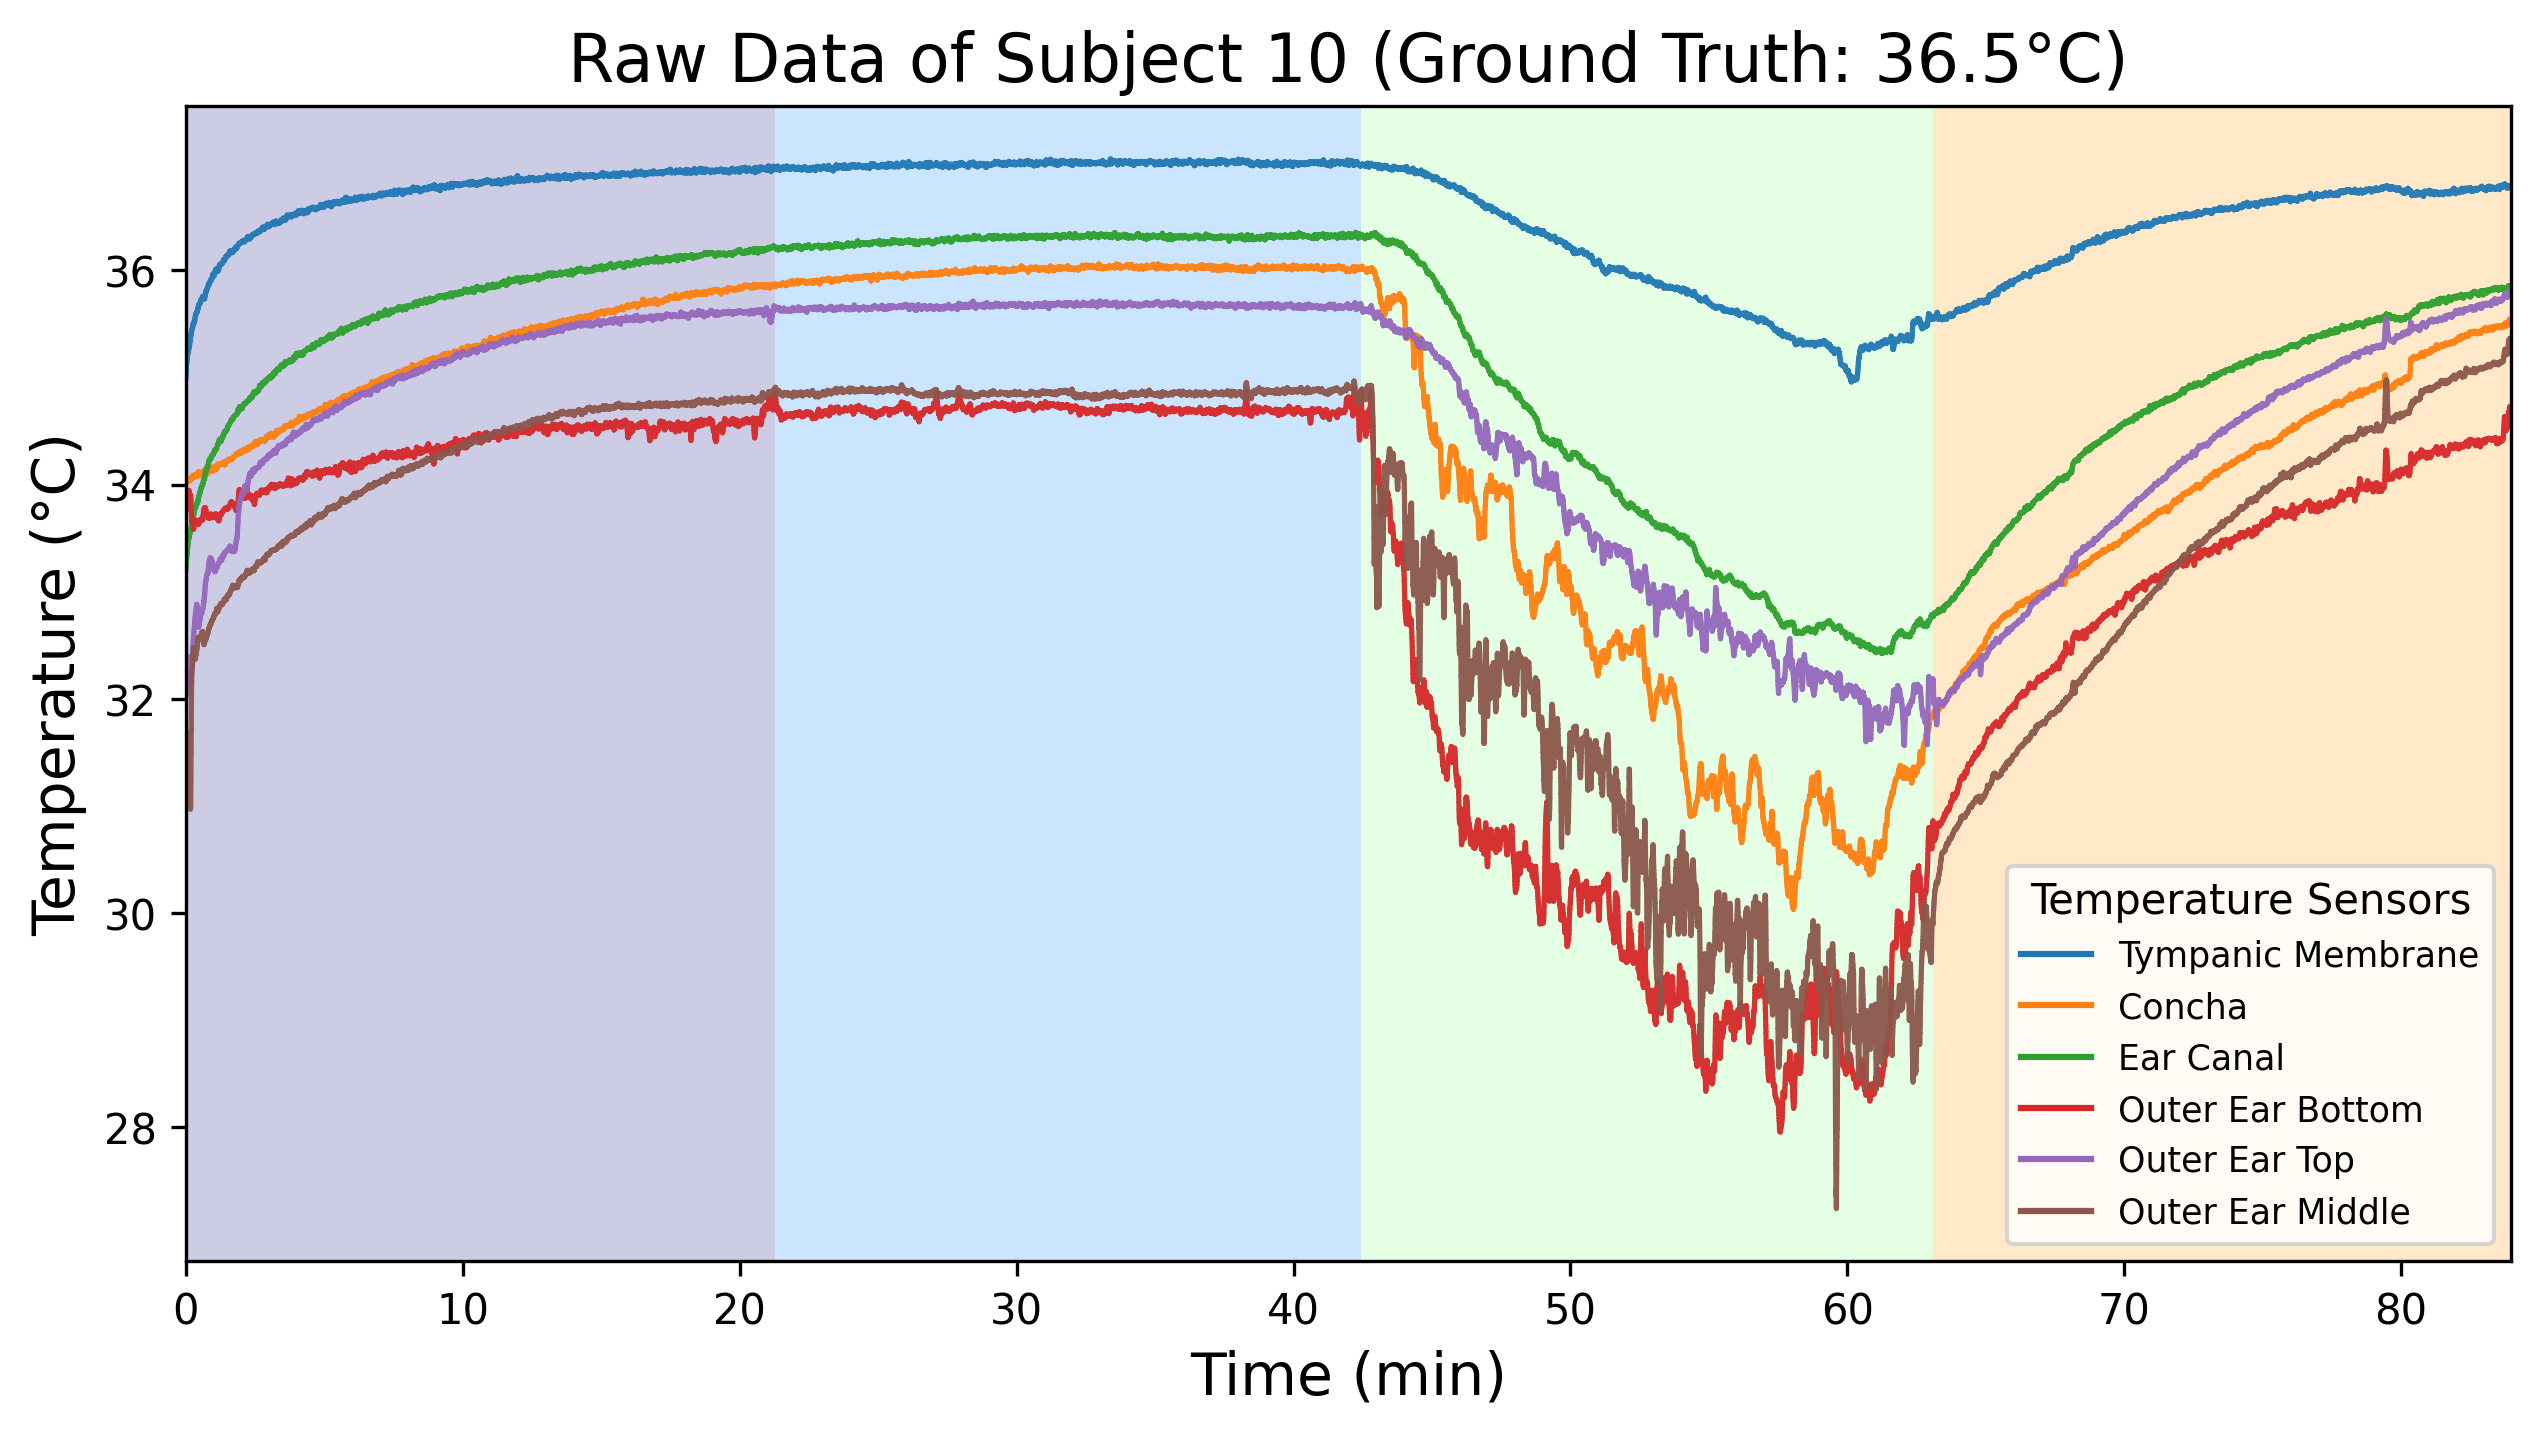
\includegraphics[width=\textwidth]{thesis-doc/images/study1/Logging_person_10_0smoothed_raw_data.png}
    \caption{Raw data of a measurement in study 1 of subject 10. The subject had a body temperature of $36.5^\circ\text{C}$ at the beginning. Phases 1-4 are shown, distinguished by the background color of the plot. In phase 1, the sensor has adjusted and acclimated to the temperature of the subject. After the sensor settled in, Phase 2 measured the temperature while sitting in a room. In phase 3, the subject went for a walk outside. In phase 4, he went back into the room to see how the sensors settled back to the calmer environmental conditions.}
    \label{fig:ch:Evaluation:Study1:RawData}
\end{figure}

\subsection{Hypothesis 1: Lower Temperature Measured on Sensors Behind the Ear}
\label{subsec:Evaluation:Study1:Hypothesis1}

The first hypothesis is to show that a lower temperature is measured behind the ear than in the ear.
For this purpose, the analysis was considered in two perspectives. 
First, only the data points where the subject was sitting were recorded, and second, all data were considered except for the acclimatization phase (phase 1).

In the first perspective, the data were considered at which the subject was seated (phase 2). 
Here, for all subjects, the mean temperature behind the ear was \(36.30^\circ\text{C}\), while the mean temperature inside the ear was \(36.74^\circ\text{C}\). 
To prove a statistically significant difference between the two means, a t-test can be used.
The t-test yielded a p-value of \(0.0424\), which is below the alpha value of \(0.05\).
Since the p-value is below the alpha, this is evidence of a significant difference.
The mean error between the ground truth and the temperature measured behind the ear was \(0.79^\circ\text{C}\), and that for the temperature in the ear was \(0.38^\circ\text{C}\). 
The p-value for the comparison of these errors was \(0.0115\), again indicating a statistically significant difference.
Thus, it is clear that temperature is measured significantly lower behind the ear than in the ear while sitting.

The second perspective now also looks at other phases of the study. 
Now, in addition to the sitting phase (phase 2), the walking phase (phase 3) and the regeneration phase (phase 4) were also considered. 
The mean temperature behind the ear was \(35.33^\circ\text{C}\) and in the ear it was \(36.02^\circ\text{C}\). 
The p-value of the T-test was \(0.0158\), which again is statistically significant.
The mean error behind the ear was \(1.67^\circ\text{C}\) and in the ear it was \(0.98^\circ\text{C}\). 
The p-value for the comparison of these errors was \(0.0158\), which is also statistically significant.

This can also be seen in Figure \ref{fig:eval:study1:hypothesis1_result}.
The two boxplot images show the sitting and walking phases (phase 2 and 3), always zeroed to the temperature measured by the thermometer before the measurement.
During sitting (phase 2), the temperature measured at the tympanic membrane is very close to the temperature measured by the thermometer ($\pm0.25^\circ\text{C}$). 
The sensors in the ear canal and pinna also show high accuracy. 
For the sensors behind the ear, although the median is sometimes very close to the sensors in the ear, the outliers are strongly represented here, which questions the reliability of the signals.
When comparing the sensors behind the ear, the sensor placed at the top behind the ear provides the best results. 
This is due to the position behind the ear, the further below the ear, the more external influences are felt, such as a gust of wind, even if only with slight movements.
This can be seen more clearly in the boxplot for phase 3, while the test subjects were out walking. 
While here also the sensor pointing to the eardrum shows the best results, all other sensors have outliers.
There is also a significant difference between the sensor in the ear canal and the auricle. 
The sensor in the ear canal is further in the ear and thus somewhat more protected from external conditions, which is also evident here. 
The findings of the boxplot from phase 2 are also confirmed for the sensors behind the ear.

The second perspective also confirms the hypothesis that the temperature measured behind the ear is statistically significantly lower than that measured in the ear. 
However, the sensors behind the ear also show a statistically significant higher error compared to the ground truth, especially when the subject is involved in activities such as walking. 
These findings have important implications for the use of ear-based temperature sensors in various applications.

\begin{figure}[!h]
    \centering
    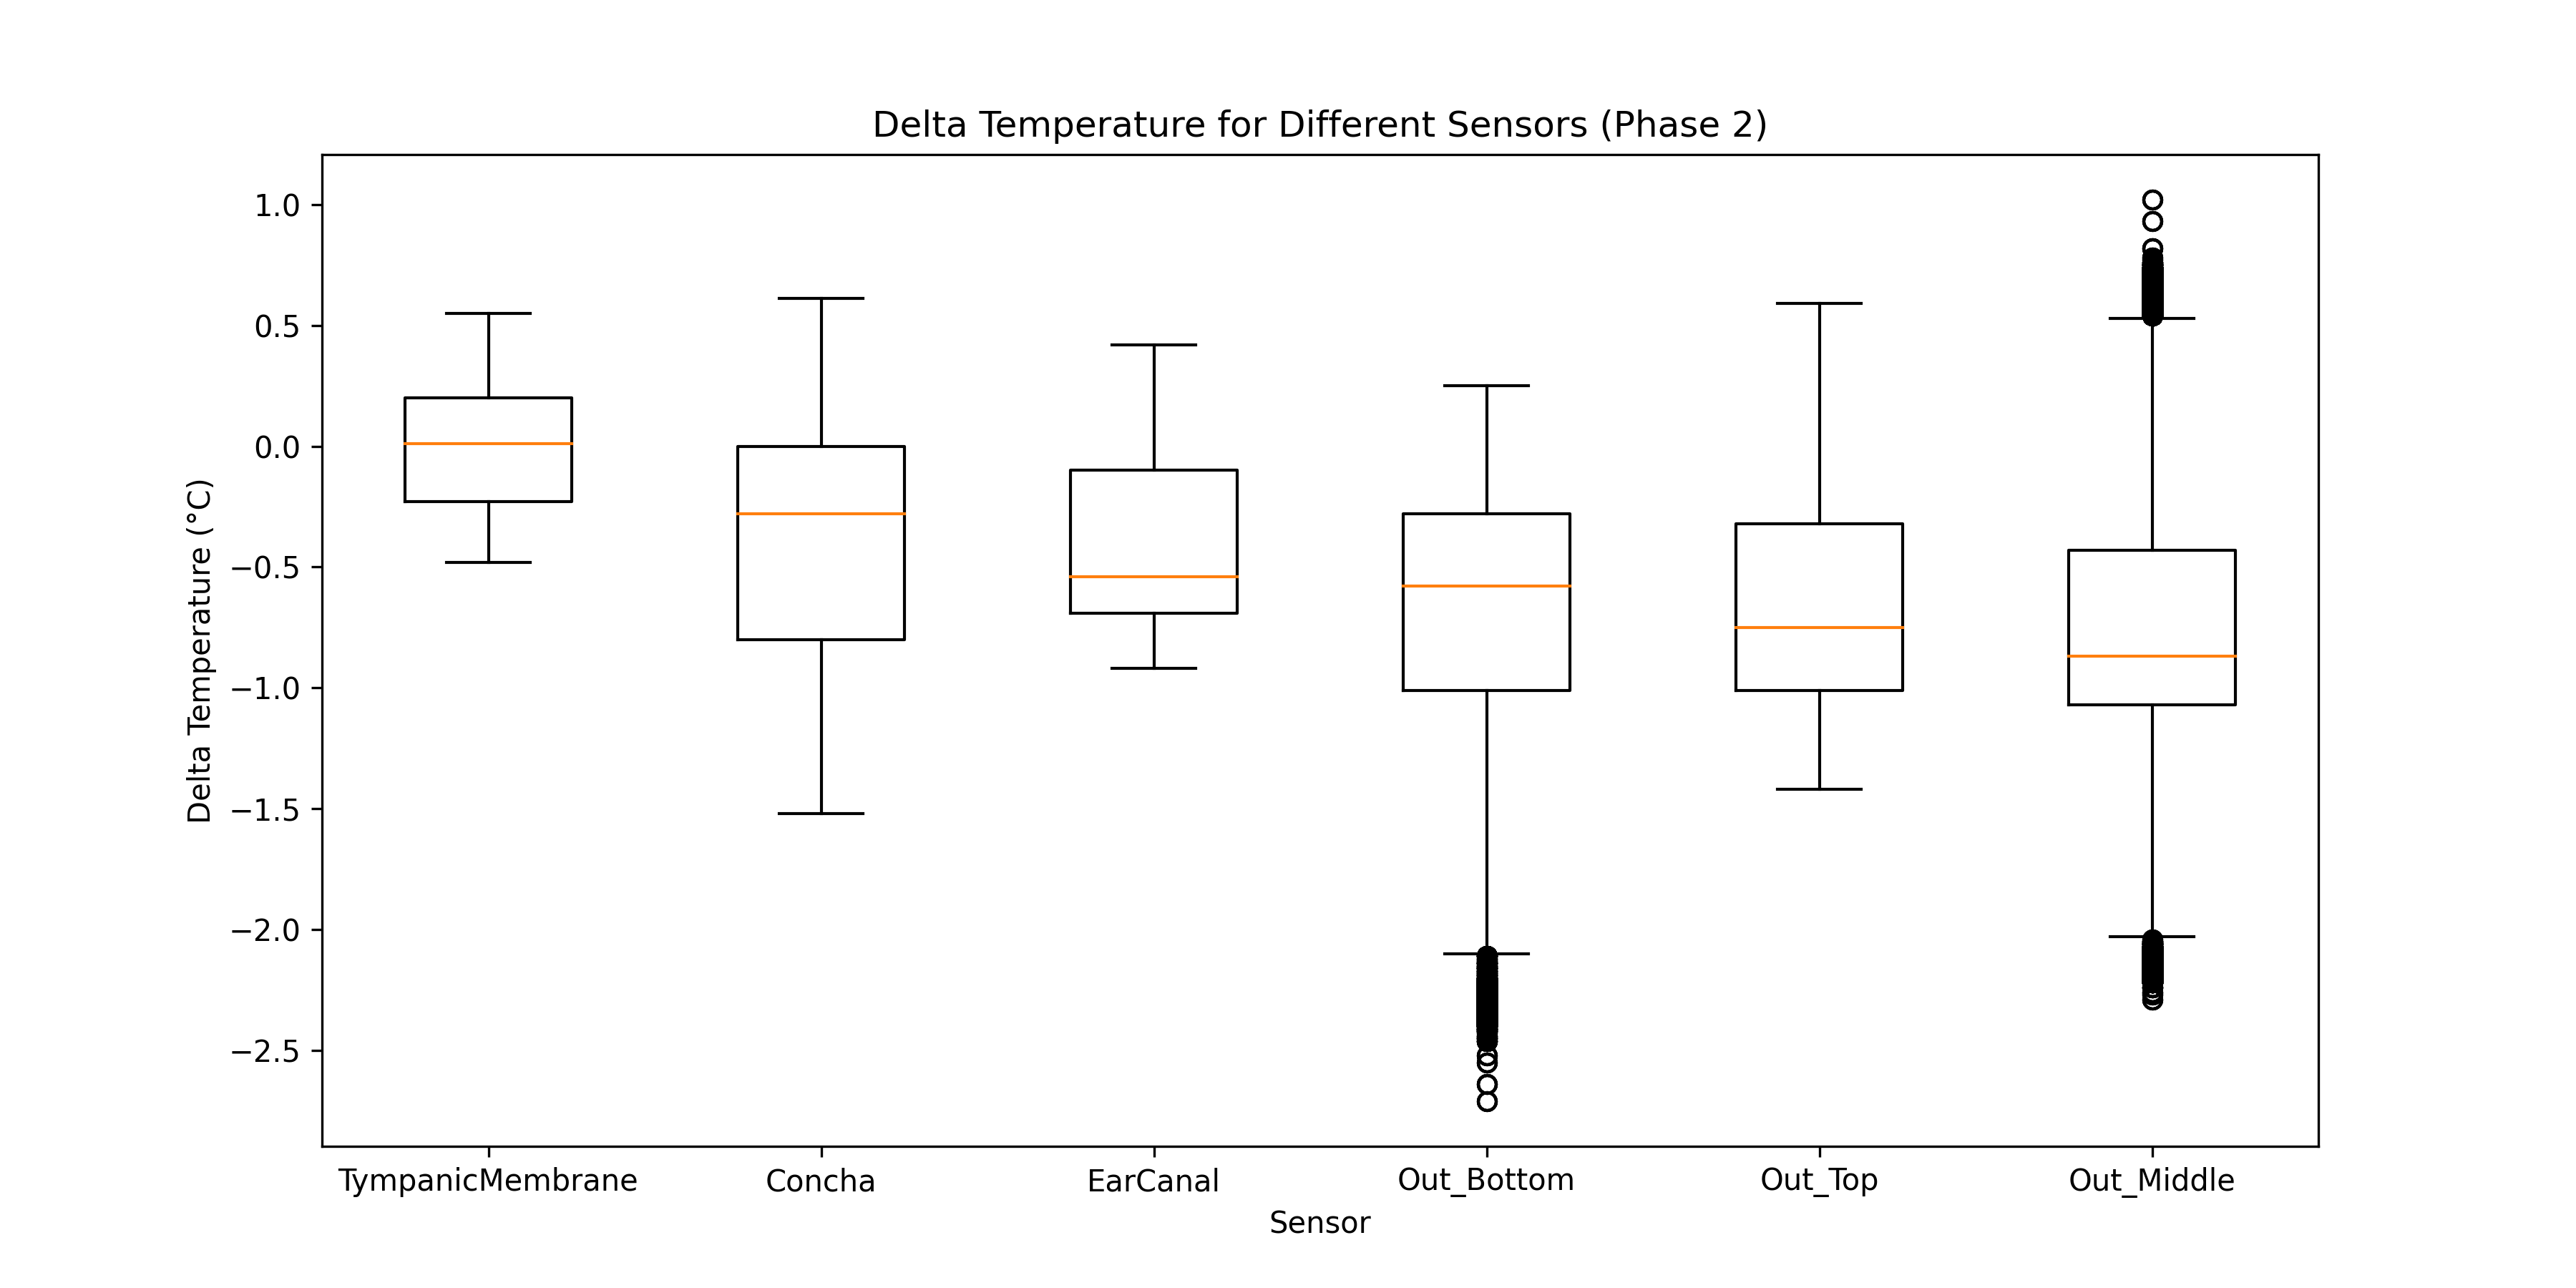
\includegraphics[width=\textwidth]{thesis-doc/images/study1/hypothesis1/hypothesis1_boxplot_phase_2.png}
    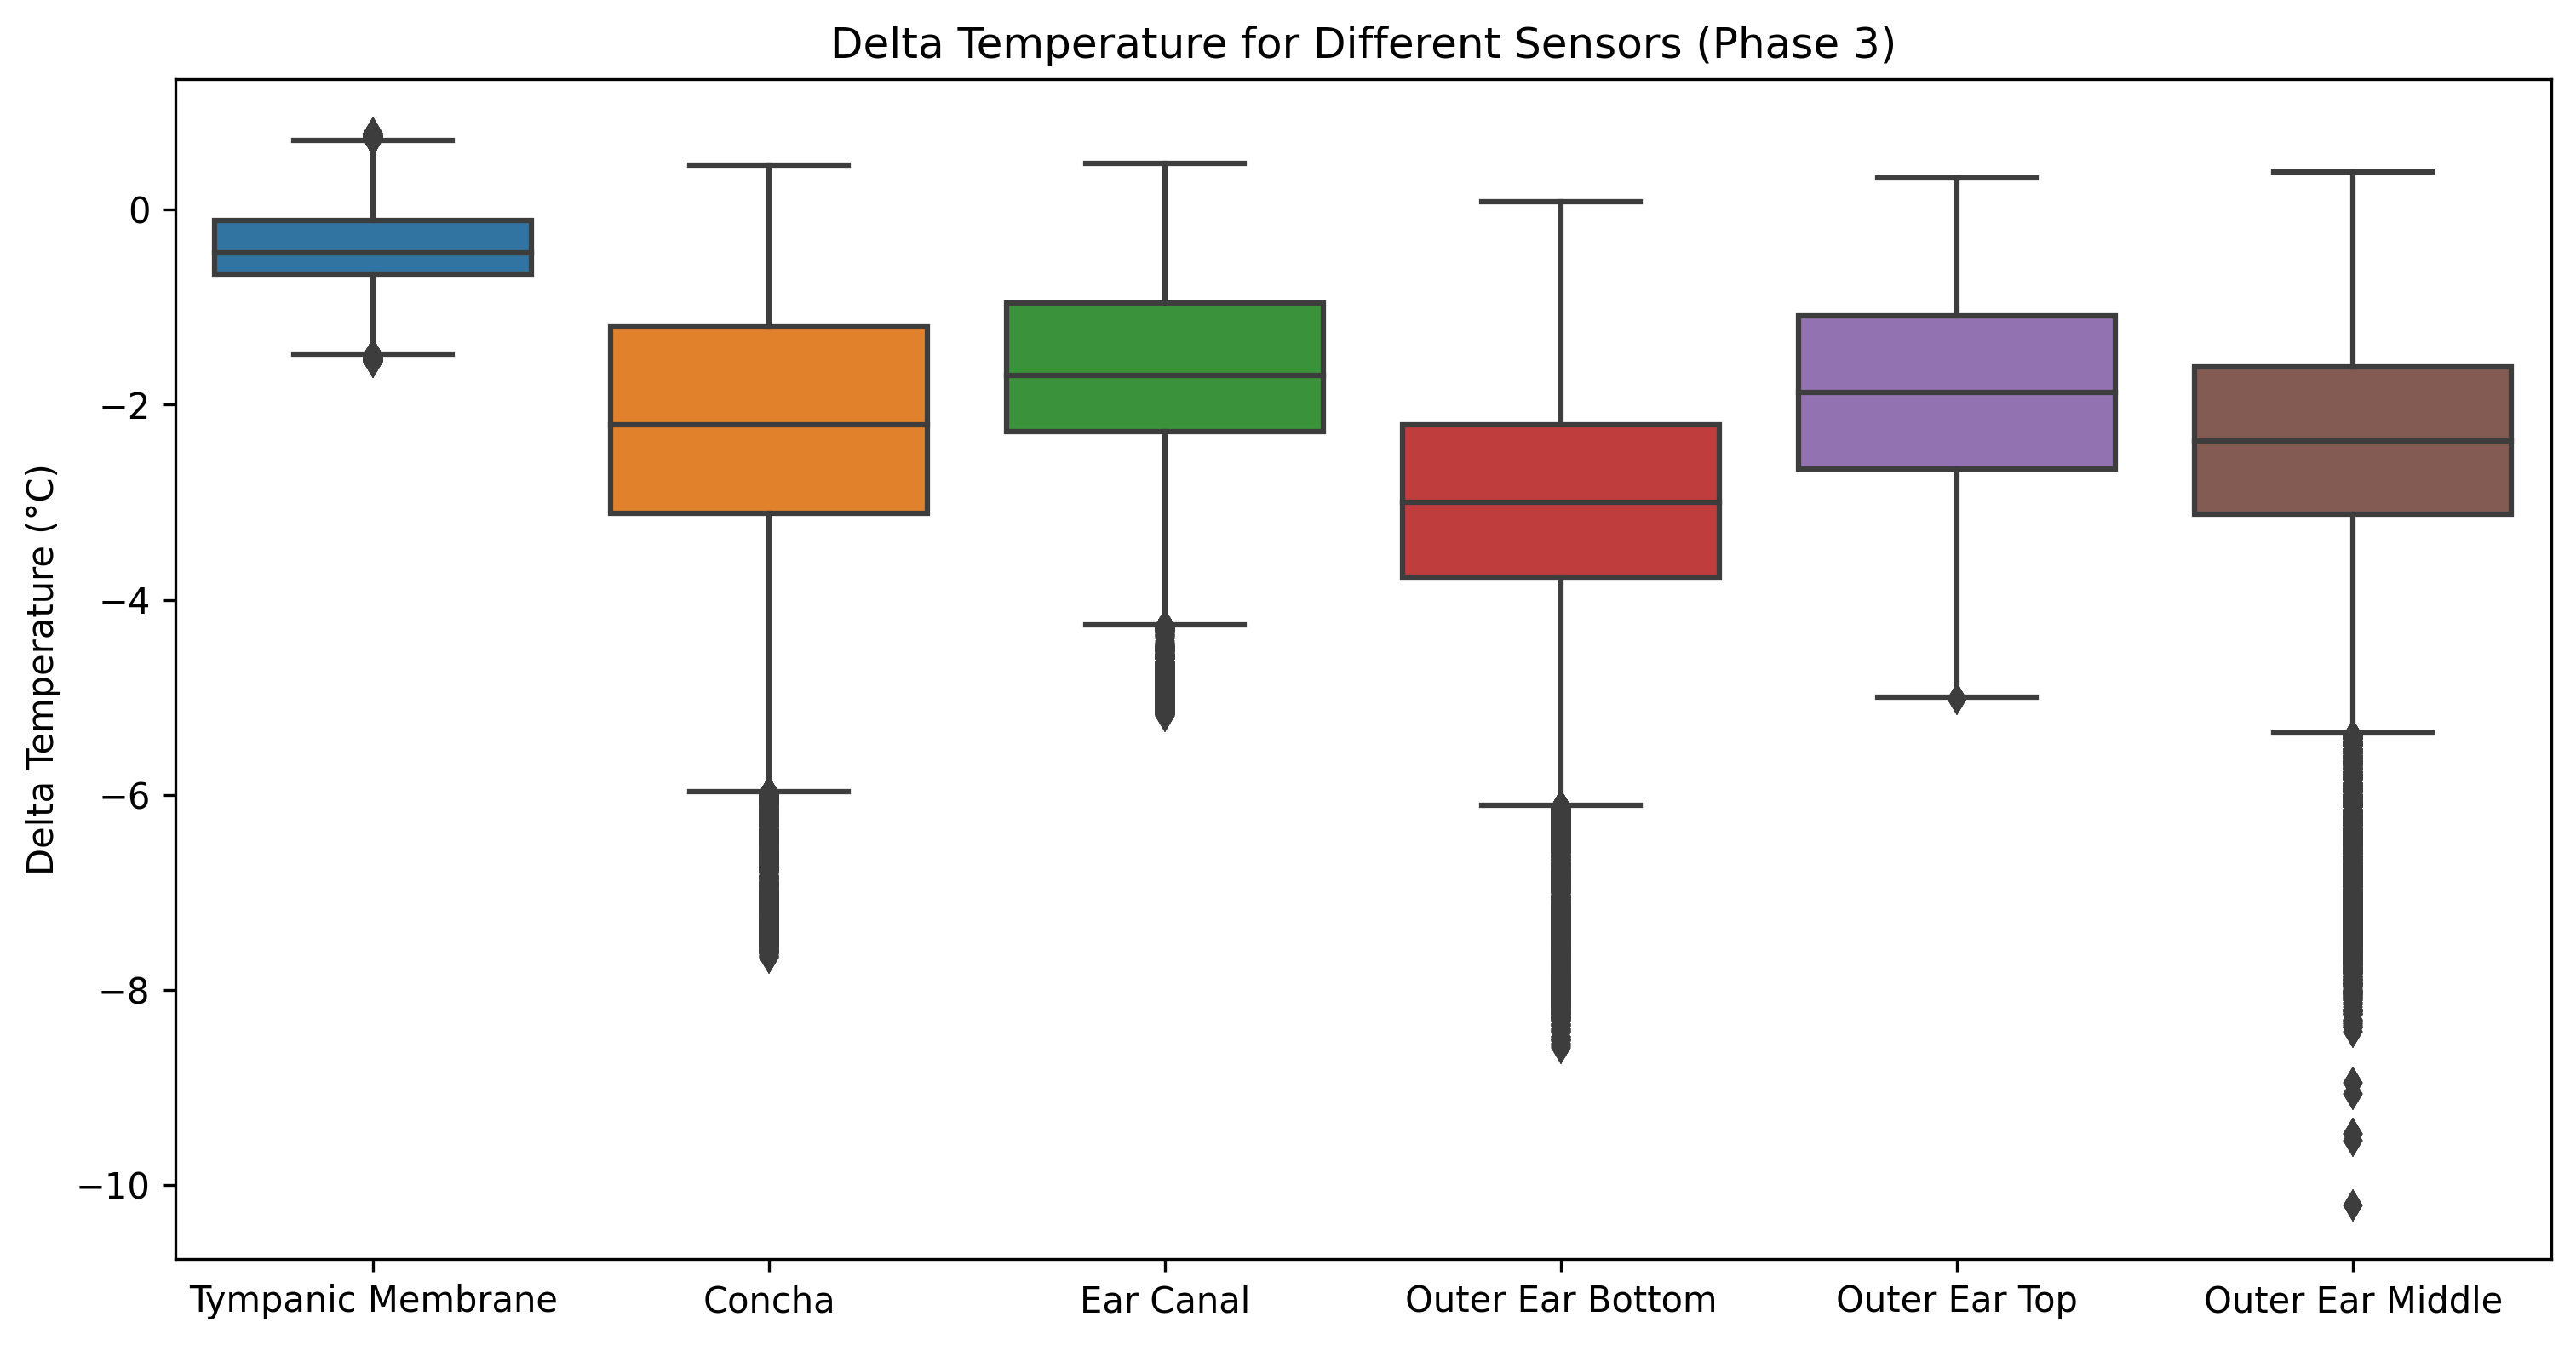
\includegraphics[width=\textwidth]{thesis-doc/images/study1/hypothesis1/hypothesis1_boxplot_phase_3.png}
    \caption{Boxplots visually illustrating the distribution of measured values from different sensor positions during phase 2 (indoor) and phase 3 (outdoor). Central tendencies and their dispersion for the analysis of the sensors under different environments can be seen. Temperature values were subtracted from the thermometer reading to compare all user data together. These visualizations are an essential part of the evaluation of Hypotheses 1 and 2, as they highlight differences in variance and highlight potential outliers.}
    \label{fig:eval:study1:hypothesis1_result}
\end{figure}

\subsection{Hypothesis 2: Variance Difference Indoor/Outdoor}
\label{subsec:Evaluation:Study2:Hypothesis2}

The second hypothesis is to show that the variance in temperature readings from ear-based sensors is lower indoors than outdoors.
This expectation is derived from the fact that the external influences in an indoor environment with closed windows are significantly less than the external influences outside during walking.
To test this hypothesis empirically, the data set of several ear-based temperature sensors at different positions was considered, both indoors and outdoors.
The different situations within the studies were divided into phases. 
Phase 2 represents an indoor measurement, and Phase 3 represents an outdoor measurement during walking.
Here, the temperature values in different areas of the ear were looked at closely.
To prove the hypothesis, the variances per temperature sensor were now calculated for phases 2 and 3 respectively. 
The results show a clear pattern. 
The mean variance for the tympanic sensor $0.00096$ indoors and \(0.107\) outdoors.
This pattern was consistently observed for other sensor locations, such as the auricle with a mean variance of $0.00307$ indoors and $1.134$ outdoors.
A detailed listing of the results can be seen in Table \ref{subsec:Evaluation:Study2:Hypothesis2:mean_variance_table}.
A two-sample T-test was used to statistically compare these variances.
The results provided clear evidence to support the hypothesis.
For example, the p-value for the tympanic sensor was significantly below the Bonferroni-corrected threshold, clearly refuting the null hypothesis.
This pattern is also seen for the other positions in and around the ear, providing extensive empirical support for the hypothesis.
In summary, the data confirm the second hypothesis: temperature measurements with ear-based sensors have significantly lower deviations when taken indoors than outdoors.

\begin{table}[t]
\centering
\begin{tabular}{|p{2.5cm}|c|c|c|c|c|c|}
\hline
\textbf{Sensor} & \multicolumn{2}{c|}{\textbf{MAD (in \(^\circ\text{C}\))}} & \multicolumn{2}{c|}{\textbf{Mean Variance}} & \multicolumn{2}{c|}{\textbf{Mean Diff. from}} \\
 & \multicolumn{2}{c|}{} & \multicolumn{2}{c|}{} & \multicolumn{2}{c|}{\textbf{Ground Truth (in \(^\circ\text{C}\))}} \\
\hline
 & \textbf{Indoor} & \textbf{Outdoor} & \textbf{Indoor} & \textbf{Outdoor} & \textbf{Indoor} & \textbf{Outdoor} \\
\hline
\textbf{Tympanic Membrane} & 0.025 & 0.258 & 0.00096 & 0.1074 & 0.0071 & -0.6077 \\
\textbf{Concha} & 0.042 & 0.820 & 0.00307 & 1.1339 & -0.3805 & -2.5609 \\
\textbf{EarCanal} & 0.030 & 0.624 & 0.00155 & 0.6456 & -0.3934 & -1.9584 \\
\textbf{Out\_Bottom} & 0.095 & 0.800 & 0.0189 & 1.1098 & -0.7439 & -3.3107 \\
\textbf{Out\_Top} & 0.062 & 0.663 & 0.00694 & 0.6499 & -0.6060 & -2.1198 \\
\textbf{Out\_Middle} & 0.101 & 0.831 & 0.0198 & 1.0982 & -0.7452 & -2.7643 \\
\hline
\end{tabular}
\caption{Mean absolute deviation (MAD), mean variance, and mean distance from ground truth for different sensors. Phases 2 (inside) and 3 (outside) were considered. All values were calculated for each sensor and averaged over all subjects.}
\label{subsec:Evaluation:Study2:Hypothesis2:mean_variance_table}
\end{table}

\subsection{Hypothesis 3: Relative Changes in Temperature Readings}
\label{subsec:Evaluation:Study1:Hypothesis3}
The third hypothesis examines the correlation between the relative changes in temperature readings from different sensor locations in Phases 2 and 3.
This is used to understand the consistency between the different sensor readings, particularly in relation to changing weather conditions.d
Mean absolute deviation is used for analysis to better understand the consistency between the different temperature sensor readings. 
Table \ref{subsec:Evaluation:Study2:Hypothesis2:mean_variance_table} shows the MAD value for each sensor location in phase 2 (indoor) and 3 (outdoor). 
Increased variance is seen in the outdoor phase. 
While the sensor measurement at the tympanic membrane is only $0.2 ^\circ\text{C}$, the other sensor locations have a mean absolute variance of about $0.6-0.8^\circ\text{C}$.
This is mainly due to the fact that external influences such as wind, rain, or sunlight may play a large role here.
When the subjects went for a walk, this was all represented, which explains the deviations here. 
This shows that these sensor positions are not as stable to external environmental influences as the sensor directed at the eardrum.
Similarly, this can be seen in the heatmap of Figure \ref{fig:eval:study1:hypothesis3_result}. 
Here, the correlations in phase 2 (indoor) and phase 3 (outdoor) have been plotted as a heatmap. 
Significant differences in the correlation of temperature values between the two phases 2 and 3 can be seen. 
In phase 2, the correlations are generally slightly lower, especially the measurement of tympanic membrane is very different from the other results.
This can be explained by variations in the subjects' sensor results, for example, when subjects readjust the sensor or move their head awkwardly, especially for the sensors behind the ear. 
In contrast, the correlations in Phase 3 are higher than average, often exceeding $0.9$. 
This suggests that all sensors respond equally to external environmental changes.
The reason for this is that during outdoor activities, conditions such as wind and sunlight affect all sensor locations equally.
This explains the sharp drop in temperature readings, resulting in high correlations.
In summary, the heat map supports the hypothesis by showing that indoor sensor readings fluctuate widely, while outdoor conditions tend to synchronize readings, albeit with higher volatility.
In summary, this hypothesis is supported by the analysis of the mean absolute deviation. 
Furthermore, it can be seen that the sensors at the different positions are differently stable to external environmental influences, especially when the subjects are outdoors.

\begin{figure}
    \centering
    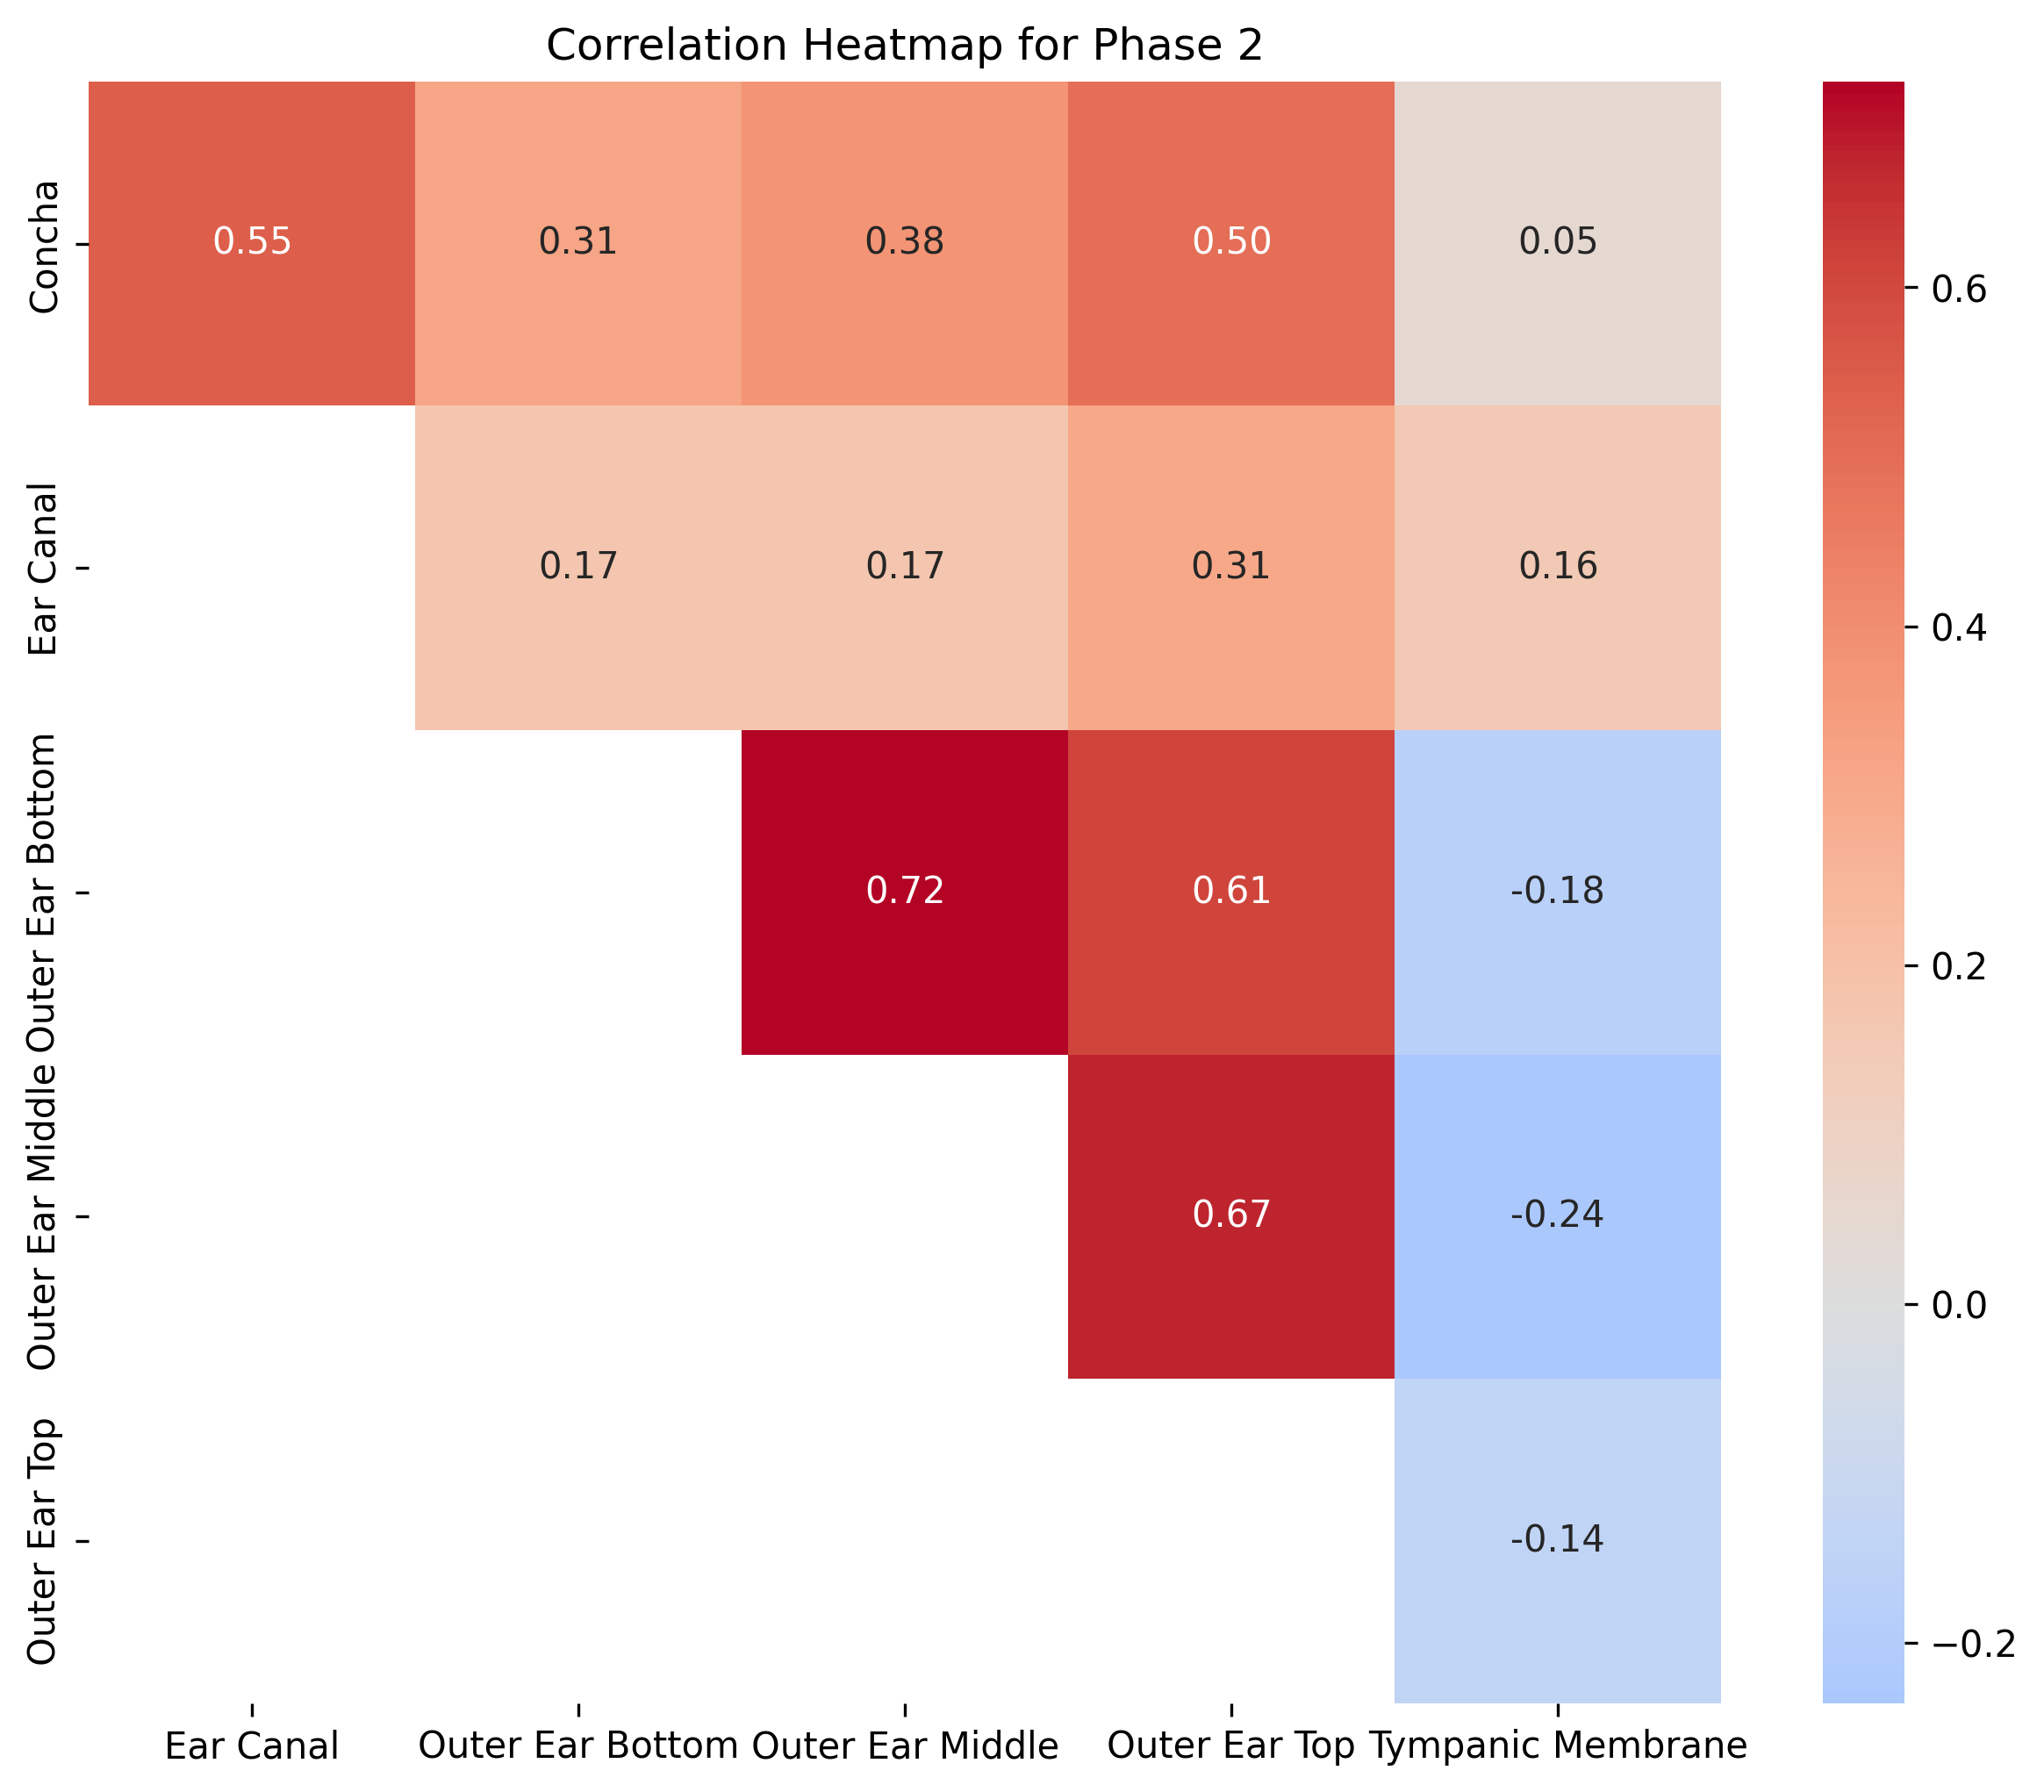
\includegraphics[width=0.9\textwidth]{thesis-doc/images/study1/hypothesis3/Correlation_Heatmap_Phase_2.png}
    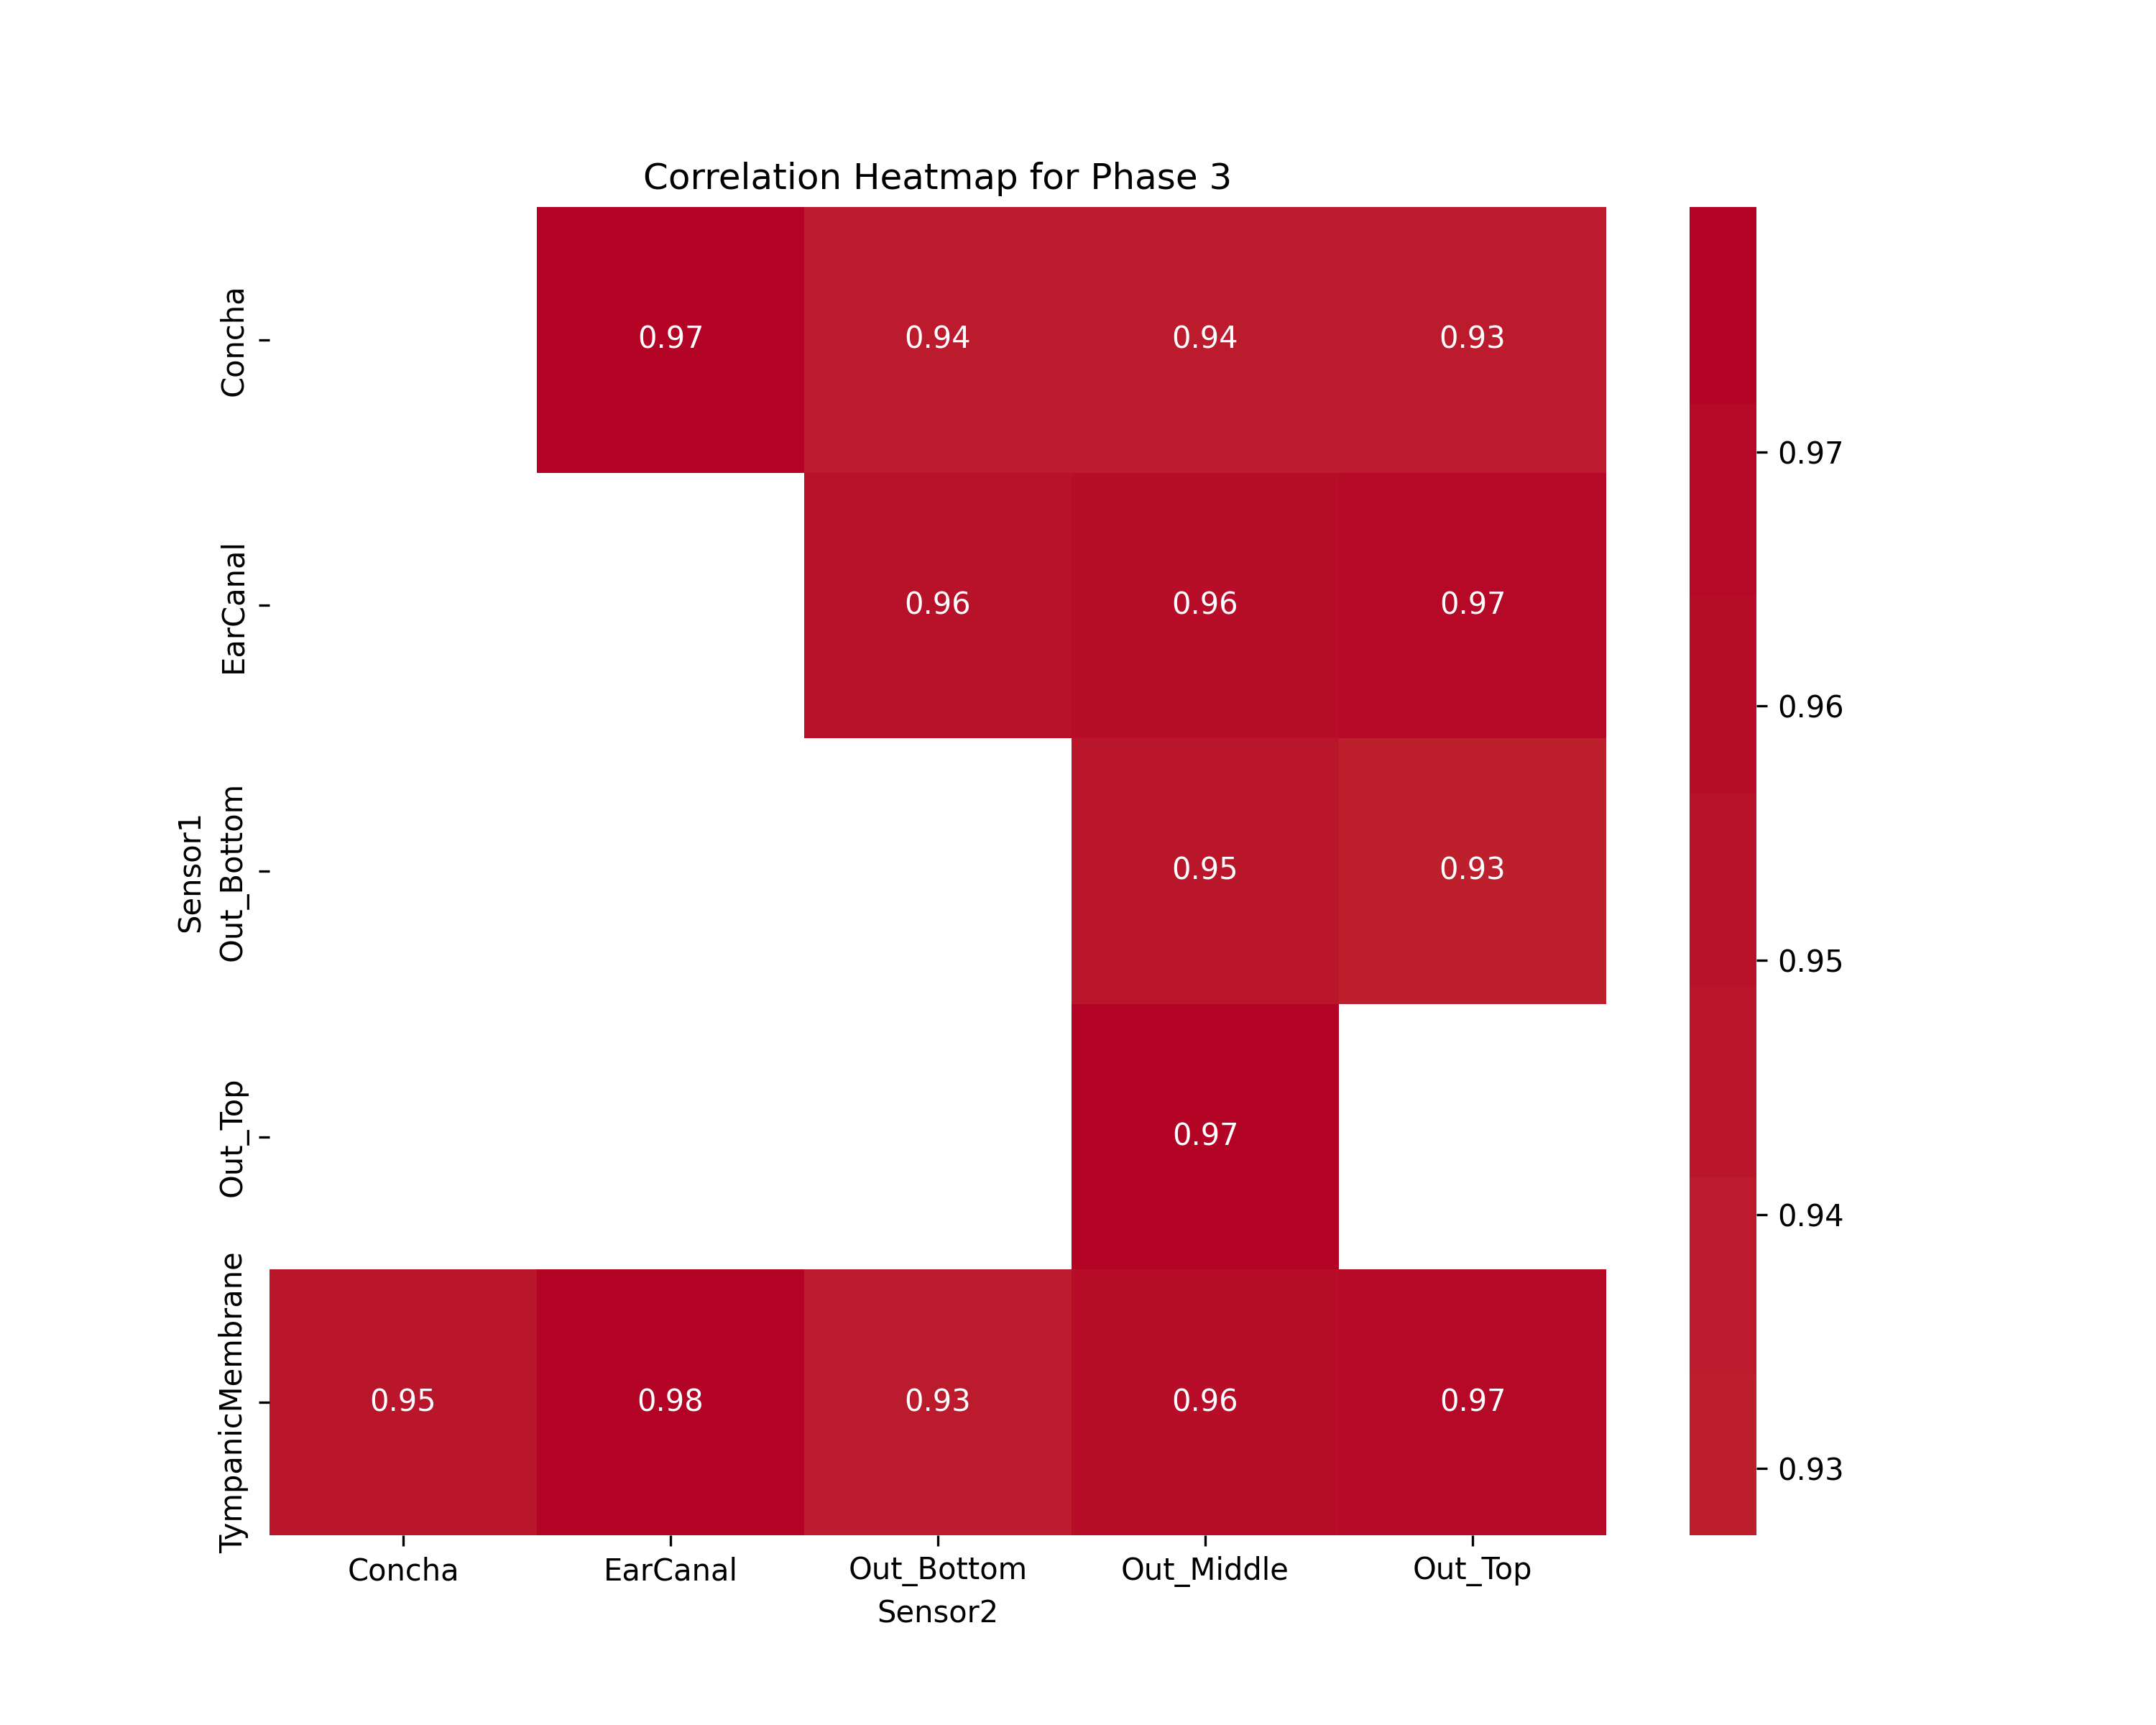
\includegraphics[width=0.9\textwidth]{thesis-doc/images/study1/hypothesis3/Correlation_Heatmap_Phase_3.png}
    \caption{Heat maps showing the correlation matrices of temperature readings from different ear-based sensors during Phase 2 (indoor) and Phase 3 (outdoor). The color-coded matrices provide a visual representation of how strongly each pair of sensors correlates under different conditions. Darker shading represents higher correlation and helps assess consistency between sensor measurements and their sensitivity to environmental changes, providing empirical evidence for Hypothesis 3.}    
    \label{fig:eval:study1:hypothesis3_result}
\end{figure}

\subsection{Hypothesis 4: Temperature at the Tympanic Membrane Is Most Stable}
\label{subsec:Evaluation:Study1:Hypothesis4}
The fifth hypothesis considers the stability of temperature sensor readings at the tympanic membrane compared to other positions during phases 2 (indoor) and 3 (outdoor).
The metric used here is the standard deviation. 
The standard deviation results can be found in Table \ref{subsec:Evaluation:Study1:Hypothesis4:std_dev_table}. 
In phase 2, the standard deviation is still relatively similar for all measurements, with only the position behind the ear in the middle yielding a worse value of $0.1154$. 
The standard deviation from the tympanic membrane nevertheless sets itself apart from those of the others with $0.0288$ compared to $0.05-0.07$. 
In phase 3, however, it is clear that the measurement of temperature at the tympanic membrane shows the most stability. 
At $0.1971$, the deviation is significantly smaller than for the rest $0.65-0.92$. 
Additionally, it can be seen from the figure \ref{fig:eval:study1:hypothesis1_result} that measurements at the tympanic membrane shows the least quantile differences and is closest to the thermometer values. 
From the calculated standard deviations, it appears that the tympanic membrane has the lowest values in both phases, indicating higher stability. 
In contrast, the other sensors show higher standard deviations, more specifically the sensors outside the ear. 
This makes them more susceptible to external conditions, such as environmental changes.
Thus, this confirms the hypothesis that the pom-pom skin provides the most stable temperature readings.

\begin{table}[t]
\centering
\begin{tabular}{|l|c|c|}
\hline
\textbf{Sensor} & \textbf{Mean Standard Deviation} & \textbf{Mean Standard Deviation} \\
& \textbf{Phase 2 (indoor)} & \textbf{Phase 3 (outdoor)} \\
\hline
\textbf{Tympanic Membrane} & 0.0308 & 0.3048 \\
\textbf{Concha} & 0.0535 & 0.9882 \\
\textbf{Ear Canal} & 0.0378 & 0.7496 \\
\textbf{Out\_Bottom} & 0.1138 & 1.0156 \\
\textbf{Out\_Top} & 0.0730 & 0.7836 \\
\textbf{Out\_Middle} & 0.1176 & 0.9875 \\
\hline
\end{tabular}
\caption{Standard deviations of temperature readings for different sensors during phases 2 and 3, averaged over all subjects. Lower values indicate higher stability.}
\label{subsec:Evaluation:Study1:Hypothesis4:std_dev_table}
\end{table}

\subsection{Hypothesis 5: Movement Leads to Changes in the Temperature Readings}
\label{subsec:Evaluation:Study1:Hypothesis5}

Hypothesis 5 states that the physical movement of the participants will have an effect on the various temperature sensors. 
This section will cover the methodology, evaluation, and discussion of this hypothesis.
To investigate the influence of exercise, both phases 2 and 3 were considered. 
In phase 2, subjects sat in a room for 20 minutes, and in phase 3, they walked outdoors for 20 minutes.
During both phases, temperature was measured at the 6 temperature sensors using $8 Hz$. 
In addition, data from the inertial measurement unit (IMU), which consists of an accelerometer, a gyroscope, and a magnetometer, were sampled at $50Hz$. 
The relative change was now calculated for each temperature sensor as follows:

\[
\text{relative change} = \left| \frac{{T_{\text{current}} - T_{\text{previous}}}}{{T_{\text{previous}}}} \right| \times 100
\]

Where \( T_{\text{current}} \) and \( T_{\text{previous}} \) are the current and previous temperature values, respectively. 
The absolute value of the relative change was taken to capture the magnitude of the change regardless of direction. 
This value was then multiplied by 100 to express it as a percentage.
In addition, the mean motion was derived from the IMU data.
For this purpose, a metric for mean motion was calculated. 
For each time point, the mean motion \(M\) was calculated using the following formula:

\[
M = \sqrt{{\sum_{i=1}^{n} x_i^2}}
\]

Where \( x_i \) is the IMU reading from one of the 9 columns (`ACC\_X`, `ACC\_Y`, `ACC\_Z`, `GYRO\_X`, `GYRO\_Y`, `GYRO\_Z`, `MAG\_X`, `MAG\_Y`, `MAG\_Z`). This approach effectively captures the total motion intensity at each time point by considering all available IMU sensors.
Figure \ref{fig:eval:study1:hypothesis5_result} shows the relative changes in each temperature sensor reading for the indoor and outdoor phases.
The movement of the subjects is shown at the bottom. 
The plots show a nuanced relationship between movement and temperature sensor values.
Relative changes can be seen for the individual temperature sensors in the two phases, but this may be due to different conditions. 
In Phase 3, temperature generally decreased significantly when subjects left the room and went outside.
This is exacerbated by movement during the outdoor phase. 

\begin{figure}
    \centering
    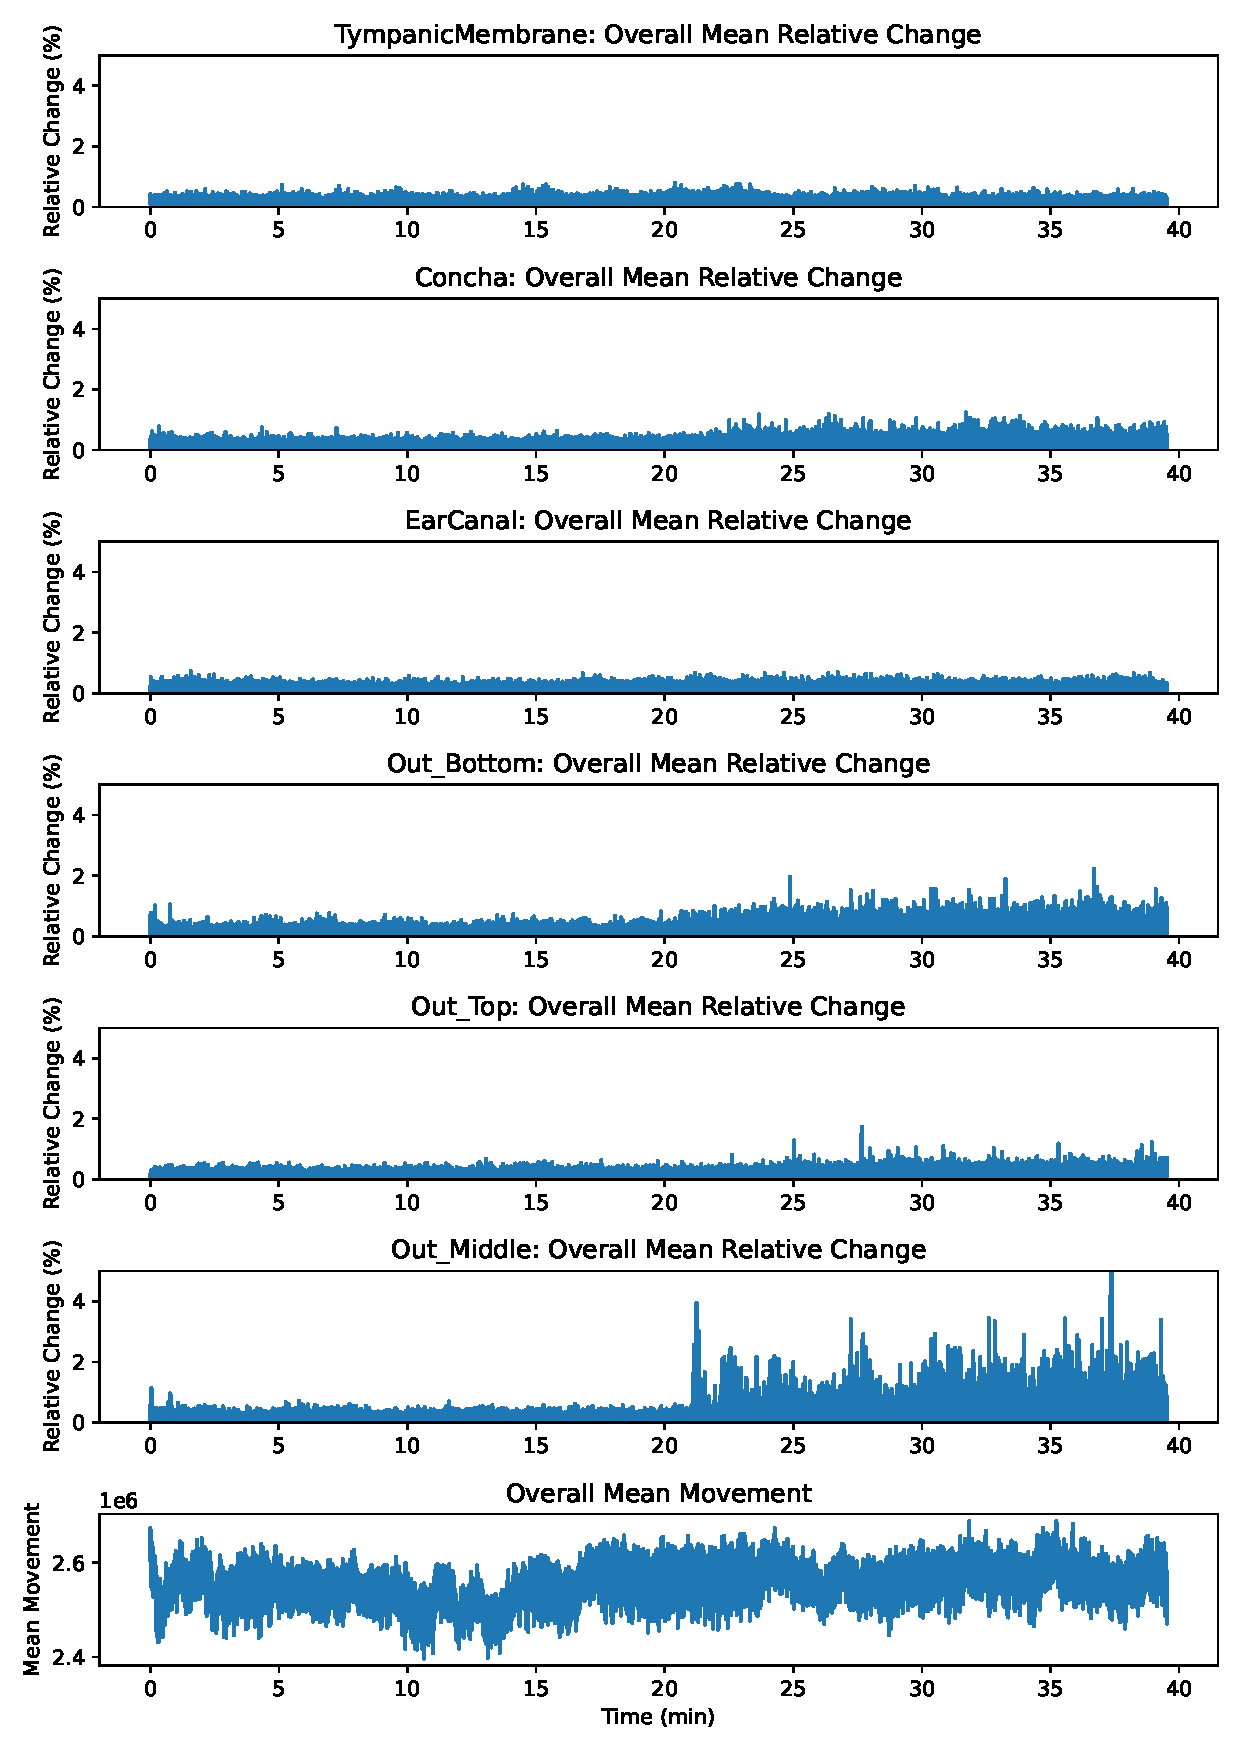
\includegraphics[width=\textwidth]{thesis-doc/images/study1/hypothesis5/overall_mean_data_hypothesis5.pdf}
    \caption{ADD DESCRIPTION}    
    \label{fig:eval:study1:hypothesis5_result}
\end{figure}


\section{Results and Discussion from Study 2}
\label{sec:Evaluation:Study2}
Having checked the validity of the temperature measurements, a second study will now observe how the measured temperature behaves when the subject is placed under stress.
A more detailed introduction to the design and objectives of study 2 is described in chapter~\ref{ch:Design:Study:Study2}.
The ground truth used here is the Polar H9, which allows an HRV measurement to be recorded.
At the beginning, it is checked whether the subjects really had stress during the study by looking at the HRV signal and classifying the stress.
Then, different hypotheses are considered and proved or disproved.

\subsection{Ground Truth: Stress Detection}
\label{subsec:Evaluation:Study2:ground_truth}
At the outset, we examine whether the study actually produced stress in the subjects. 
This is necessary because the stress detection procedures used, although scientifically accepted, do not produce good results in every subject. 
A much better stress test would be the Trier Social Stress Test (TSST), but there is not enough time for this master thesis. 
As ground truth HRV (heart rate variability) values were recorded with the Polar H9.
These are saved in the form of a txt file, in which the RR intervals (resting rate) were persisted.
With this information all values needed for the classification of stress can be calculated.
These include SDNN (Standard Deviation of NN intervals), RMSSD (Root Mean Square of Successive Differences) and LF/HF (Low Frequency/High Frequency).
The SDNN represents the variability in the time between successive heartbeats (NN intervals). 
Higher SDNN often indicates better autonomic flexibility, although it may increase or decrease under stress depending on individual variability.
The RMSSD is another HRV metric for the classification of short-term variations in heart rate.
In general, higher RMSSD values represent a healthier heart and lower stress.
However, this can vary from person to person.
The LF/HF ratio is a widely used analysis method to describe the balance between parasympathetic and sympathetic activities. 
Higher values often describe the dominance of sympathetic activity, i.e. stress. 
Lower values rather describe the dominance of the parasympathetic activity, i.e. relaxation.
In addition, other measures were considered using the "KubiusHRV Standard" software.
The software provides the parameters SNS index (Sympathetic Nervous System), PNS index (Parasympathetic Nervous System) and a stress index, which should confirm the findings from SDNN, RMSSD and LF/HF ratio.
The SNS index describes the activities of the Sympathetic Nervous System. 
Higher positive values induce stress or fight-or-flight responses.
The PNS index describes the activities of the parasympathetic nervous system. 
Higher positive values indicate relaxation.
This resulted in the results shown in Table \ref{subsec:Evaluation:Study2:ground_truth_result}. 

Here it can be seen that in subject 1 the SDNN and RMSSD value decreased during the stress phase, which is an indication of stress.
However, in subject 1 there is also a decrease in LF/HF ratio, which is contrary to a normal stress phase.
The two SNS and PNS indices are helpful here, as values indicate stress, as does the stress index, which increases from 7 to 11.
In test person 2, a slight increase in the values can be seen in the stress phase, which is contrary to the expectation of recognizing stress.
The stress index also remains stable at the value 8, which confirms the values. 
The PNS and SNS indices show slight increases, which could indicate stress, but the increases are not sufficient to detect a stronger tendency here. 
In test person 3, no stress can be detected on the basis of the SDNN and RMSSD values either, as an increase in the SDNN and a decrease in the RMSSD values can be seen here. 
However, the LF/HF ratio increases, which indicates stress, as does the slight decrease in the PNS index and slight increase in the stress index to 14. 
However, the decrease in the SNS index is an atypical sign of stress, which is why stress cannot be accurately attributed to subject 3 either.
Proband 4 delivers the best values.
Here a significant decrease of the SDNN and RMSSD values during the stress phase, a dramatic increase of the LF/HF ratio, a strongly increasing stress index to 14 and changing PNS and SNS indices can be seen, which are all clear findings for stress.
Subject 4 here provides exactly the expected responses to stress.
Subject 5, on the other hand, shows a decrease in SDNN and RMSSD during the stress phase. 
This indicates stress, which is confirmed by the slight increase in the LF/HF ratio.
However, the stress index remained stable in subject 5, and the PNS and SNS index increased slightly, which is additionally indicative of stress, even though the increases are very small.

In summary, the study showed mixed efficacy in eliciting stress in the subjects, with subject 4 showing the most consistent and significant signs of stress across all measures. Interestingly, the male subjects (1, 4, and 5) generally showed more significant signs of stress compared to the female subjects (2 and 3) who showed ambiguous or inconsistent markers. This suggests that gender plays a role in these physiological responses, although further studies would be needed to confirm this hypothesis.

\begin{table}[t]
\centering
\resizebox{\textwidth}{!}{%
\begin{tabularx}{1.2\textwidth}{|c|*{12}{>{\centering\arraybackslash}X|}}
\hline
\textbf{Subj.} & \multicolumn{2}{c|}{\textbf{SDNN}} & \multicolumn{2}{c|}{\textbf{RMSSD}} & \multicolumn{2}{c|}{\textbf{LF/HF}} & \multicolumn{2}{c|}{\textbf{Stress-Index}} & \multicolumn{2}{c|}{\textbf{PNS Index}} & \multicolumn{2}{c|}{\textbf{SNS Index}} \\
 & \textbf{Sit} & \textbf{Stress} & \textbf{Sit} & \textbf{Stress} & \textbf{Sit} & \textbf{Stress} & \textbf{Sit} & \textbf{Stress} & \textbf{Sit} & \textbf{Stress} & \textbf{Sit} & \textbf{Stress} \\
\hline
1 & 65.89 & 47.25 & 29.66 & 21.99 & 12.08 & 9.80 & 7 & 11 & -1.6 & -1.85 & 1.96 & 2.73 \\
2 & 70.93 & 71.62 & 42.05 & 44.76 & 2.75 & 3.49 & 8 & 8 & -0.92 & -0.98 & 0.87 & 1.02 \\
3 & 150.45 & 163.09 & 99.82 & 79.58 & 0.68 & 1.22 & 5 & 6 & 2.21 & 0.92 & -1.33 & -0.51 \\
4 & 101.44 & 71.71 & 35.86 & 19.37 & 2.08 & 4.40 & 9 & 14 & -0.51 & -2.01 & 0.33 & 2.73 \\
5 & 225.16 & 202.75 & 268.12 & 235.46 & 0.29 & 0.34 & 2 & 2 & 7.26 & 6.44 & -2.28 & -2.24 \\
\hline
\end{tabularx}%
}
\caption{Comparison of heart rate variability (HRV) between sedentary and stressful conditions in five subjects. SDNN, RMSSD, and LF/HF are HRV metrics, while stress index, PNS index, and SNS index are derived from analysis using "KubiosHRV Standard" software. All metrics are presented as pairs, with the seated value appearing first, followed by the value under stressful conditions. The PNS is the regeneration index and indicates the recovery ability. The lower the value, the higher the regeneration phase and the more stressed the person is, the normal value is 0.
The SNS is the stress index, the higher this value, the higher the stress and correspondingly the more stressed the person is, again the normal value is 0.}
\label{subsec:Evaluation:Study2:ground_truth_result}
\end{table}

\subsection{Hypothesis 1: Measurable Temperature Rise During Stress}
\label{subsec:Evaluation:Study2:Hypothesis1}
To evaluate hypothesis 1, the analysis focuses on the average temperature changes measured by different ear-based sensors during three different phases: Sitting, Stress, and Relaxation. 
The first phase, used to acclimate the temperature sensors, is discarded here for analysis.
To ensure a fair comparison, the mean temperatures were subtracted with the ground truth for each participant.

For the dataset that includes all participants (Table \ref{subsec:Evaluation:Study2:Hypothesis1:combined_mean_temps}), the results show minimal temperature variation between phases for all sensors. 
The T-test results (Table \ref{subsec:Evaluation:Study2:Hypothesis1:TTest_Results}) are used to ensure the significance of the detectable differences.
Mean tympanic membrane temperature shows a slight decrease in mean temperature from the sitting phase $(0.06^\circ \text{C})$ to the stress phase ($0.03^\circ \text{C}$), which contradicts the hypothesis, but the T test shows statistical significance for this transition in both the overall group (P=0.049) and the subgroup of participants 1,4,5 (P=0.007). 
The sensors behind the ear (top and bottom) also show statistical significance only at the transition from sitting to weight-bearing for all participants (P=0.009 and P=0.005, respectively), whereas the middle sensor behind the ear shows marginal significance at the same transition (P=0.029).

In the subset of participants who showed significant stress responses (Table \ref{subsec:Evaluation:Study2:Hypothesis1:combined_mean_temps}), mean tympanic membrane sensor temperature also decreases slightly from the sitting to the stress phase, similar to the larger data set. 
Interestingly, the concha sensor shows an opposite pattern: temperature actually increases slightly during the stress phase.

In summary, the data do not provide clear evidence for the hypothesis. 
While there are minor variations, they are not consistently in the direction of a temperature increase during the stress phase, making it difficult to definitively confirm the hypothesis. 
It is important to note here that the implementation of the study is also a critical factor here. 
Since the study was implemented in a short time frame, which did not allow for a TSST stress test, and additionally only 5 subjects were brought in for the study, a re-study in a larger sample size is recommended to reach a more conclusive verdict.

\begin{figure}[ht]
    \centering
    
    \begin{subtable}{\textwidth}
        \centering
        \begin{tabularx}{\textwidth}{|l|*{6}{>{\centering\arraybackslash}X|}}
        \hline
        & \multicolumn{2}{c|}{\textbf{Sitting Phase}} & \multicolumn{2}{c|}{\textbf{Stress Phase}} & \multicolumn{2}{c|}{\textbf{Relax Phase}} \\
        & \textbf{All} & \textbf{1,4,5} & \textbf{All} & \textbf{1,4,5} & \textbf{All} & \textbf{1,4,5} \\
        \textbf{Sensor} & \textbf{(in $^\circ \text{C}$)} & \textbf{(in $^\circ \text{C}$)} & \textbf{(in $^\circ \text{C}$)} & \textbf{(in $^\circ \text{C}$)} & \textbf{(in $^\circ \text{C}$)} & \textbf{(in $^\circ \text{C}$)} \\
        \hline
        \textbf{TympanicMembrane} & 0.06 & 0.15 & 0.03 & 0.11 & -0.01 & 0.06 \\
        \textbf{Concha} & -0.59 & -0.02 & -0.49 & 0.01 & -0.46 & -0.01 \\
        \textbf{EarCanal} & -0.45 & -0.08 & -0.41 & -0.12 & -0.38 & -0.15 \\
        \textbf{Out\_Bottom} & -0.99 & -0.72 & -0.83 & -0.55 & -0.8 & -0.61 \\
        \textbf{Out\_Top} & -0.45 & -0.27 & -0.36 & -0.19 & -0.37 & -0.22 \\
        \textbf{Out\_Middle} & -0.79 & -0.67 & -0.61 & -0.46 & -0.59 & -0.51 \\
        \hline
        \end{tabularx}
        \caption{Mean Temperature of each phase over all participants and over participants 1,4, and 5. The measured ground truth values are subtracted from each participant's temperature data to combine the results in a more fair way.}
        \label{subsec:Evaluation:Study2:Hypothesis1:combined_mean_temps}
    \end{subtable}
    
    \vspace{1em} % Add some vertical spacing between the tables
    
    \begin{subtable}{\textwidth}
        \centering
        \resizebox{\textwidth}{!}{%
        \begin{tabularx}{1.2\textwidth}{|l|*{8}{>{\centering\arraybackslash}X|}}
        \hline
        \textbf{Sensor} & \multicolumn{4}{c|}{\textbf{Sitting - Stress}} & \multicolumn{4}{c|}{\textbf{Stress - Relax}} \\
         & \multicolumn{2}{c|}{\textbf{All}} & \multicolumn{2}{c|}{\textbf{1,4,5}} & \multicolumn{2}{c|}{\textbf{All}} & \multicolumn{2}{c|}{\textbf{1,4,5}} \\
         & \textbf{T} & \textbf{P} & \textbf{T} & \textbf{P} & \textbf{T} & \textbf{P} & \textbf{T} & \textbf{P} \\
        \hline
        \textbf{TympanicMembrane} & 2.801 & 0.049 & 11.782 & 0.007 & 0.971 & 0.387 & 0.753 & 0.530 \\
        \textbf{Concha} & -2.174 & 0.095 & -0.951 & 0.442 & -0.647 & 0.553 & 0.243 & 0.831 \\
        \textbf{EarCanal} & -0.733 & 0.504 & 2.949 & 0.098 & -0.622 & 0.568 & 0.392 & 0.733 \\
        \textbf{Out\_Bottom} & -4.728 & 0.009 & -2.723 & 0.113 & -0.444 & 0.680 & 0.863 & 0.479 \\
        \textbf{Out\_Top} & -5.692 & 0.005 & -3.178 & 0.086 & 0.430 & 0.689 & 1.880 & 0.201 \\
        \textbf{Out\_Middle} & -3.323 & 0.029 & -3.394 & 0.077 & -0.544 & 0.616 & 3.492 & 0.073 \\
        \hline
        \end{tabularx}%
        }
        \caption{T-Test results for different sensors across phases for all subjects and for subjects 1,4,5. The T-statistic and P-value for transitions between Sitting - Stress and Stress - Relax are presented.}
        \label{subsec:Evaluation:Study2:Hypothesis1:TTest_Results}
    \end{subtable}
    \caption{Evaluation results of hypothesis 1 including Mean temperatures in the Sit, Stress and Relax phases with all subjects and additionally subjects 1, 4 and 5, as only these showed stress responses in Ground Truth. For this purpose, the results of the significance test are listed to show their significance.}
    \label{sec:Evaluation:Study2:Hypothesis1:Summary}
\end{figure}

\subsection{Hypothesis 2: Variability in Temperature Changes Across Different Stress Tests}
\label{subsec:Evaluation:Study2:Hypothesis2}
Hypothesis 2 states that the temperature changes between the different stress tests. 
This can happen because stress is triggered by the sympathetic nervous system when the body enters fight-or-flight mode.
This may be addressed differently during the different stress tests, which is then reflected in the body temperature.
Hypothesis 2 is evaluated using the mean temperatures and T-test results, as shown in Figure \ref{sec:Evaluation:Study2:Hypothesis2:Summary}. 

For the mean temperatures (see Table \ref{subsec:Evaluation:Study2:Hypothesis2:combined_mean_temps}), it can be seen that the TympanicMembrane sensor showed a slight increase in temperature across all stress tests for all participants and especially for participants 1, 4, and 5. In contrast, most of the other sensors showed temperature decreases.
The T-test results (see Table \ref{subsec:Evaluation:Study2:Hypothesis1:TTest_Results}) provide interesting insights into the variability of temperature changes across different stress tests. 
The Out\_Bottom sensor showed significant differences ($p<0.05$) in transitions between Stroop-N-Back and N-Back Math for all participants, providing strong evidence of variability. 
However, the TympanicMembrane and EarCanal sensors did not show statistically significant results, indicating a relatively consistent pattern of temperature change across all stress tests.
Since it was already evident from previous studies that the signal on the tympanic membrane is the most accurate, no pattern is apparent in this small sample size.
For the subset of participants 1, 4, and 5, the T-test results show similar trends but are generally less significant due to the smaller sample size.

Overall, the results partially support hypothesis 2 by indicating significant variability in temperature changes across different stress tests, particularly for certain sensors. 
However, these are not consistent across multiple sensors. 
However, the lack of significance for some sensors suggests that further investigation is needed to definitively confirm this hypothesis, in detail a higher crosscheck sample size.

\begin{figure}[ht]
    \centering
    % First Table: Mean Temperatures
    \begin{subtable}{\textwidth}
        \centering
        \begin{tabularx}{\textwidth}{|l|*{6}{>{\centering\arraybackslash}X|}}
        \hline
        & \multicolumn{2}{c|}{\textbf{Stroop Test}} & \multicolumn{2}{c|}{\textbf{N-Back Test}} & \multicolumn{2}{c|}{\textbf{Math Test}} \\
        & \textbf{All} & \textbf{1,4,5} & \textbf{All} & \textbf{1,4,5} & \textbf{All} & \textbf{1,4,5} \\
        \textbf{Sensor} & \textbf{(in $^\circ \text{C}$)} & \textbf{(in $^\circ \text{C}$)} & \textbf{(in $^\circ \text{C}$)} & \textbf{(in $^\circ \text{C}$)} & \textbf{(in $^\circ \text{C}$)} & \textbf{(in $^\circ \text{C}$)} \\
        \hline
        \textbf{TympanicMembrane} & 0.06 & 0.15 & 0.03 & 0.12 & 0.02 & 0.09 \\
        \textbf{Concha} & -0.53 & 0.0 & -0.5 & 0.02 & -0.46 & 0.01 \\
        \textbf{EarCanal} & -0.4 & -0.07 & -0.42 & -0.1 & -0.4 & -0.14 \\
        \textbf{Out\_Bottom} & -0.9 & -0.63 & -0.84 & -0.57 & -0.79 & -0.52 \\
        \textbf{Out\_Top} & -0.43 & -0.25 & -0.37 & -0.19 & -0.33 & -0.18 \\
        \textbf{Out\_Middle} & -0.71 & -0.55 & -0.63 & -0.47 & -0.56 & -0.44 \\
        \hline
        \end{tabularx}
        \caption{Mean Temperature of each stress test over all participants and over participants 1,4, and 5. The measured ground truth values are subtracted from each participant's temperature data to combine the results in a more fair way.}
        \label{subsec:Evaluation:Study2:Hypothesis2:combined_mean_temps}
    \end{subtable}

    \vspace{1em} % Add some vertical spacing between the tables

    % Second Table: T-Tests
    \begin{subtable}{\textwidth}
    \centering
    \resizebox{\textwidth}{!}{%
    \begin{tabularx}{1.2\textwidth}{|l|*{8}{>{\centering\arraybackslash}X|}}  % Changed 8 to 9
    \hline
    \textbf{Sensor} & \multicolumn{4}{c|}{\textbf{Stroop-N-Back}} & \multicolumn{4}{c|}{\textbf{N-Back-Math}} \\
    
    & \multicolumn{2}{c|}{\textbf{All}} & \multicolumn{2}{c|}{\textbf{1,4,5}} & \multicolumn{2}{c|}{\textbf{All}} & \multicolumn{2}{c|}{\textbf{1,4,5}} \\
    
    & \textbf{T} & \textbf{p} & \textbf{T} & \textbf{p} & \textbf{T} & \textbf{p} & \textbf{T} & \textbf{p} \\
    \hline
    \textbf{TympanicMembrane} & 1.51 & 0.20 & 1.31 & 0.32 & 0.80 & 0.47 & 0.97 & 0.43 \\
    \textbf{Concha} & -2.65 & 0.06 & -1.25 & 0.34 & -1.34 & 0.25 & 0.20 & 0.86 \\
    \textbf{EarCanal} & 1.57 & 0.19 & 2.30 & 0.15 & -0.45 & 0.68 & 2.62 & 0.12 \\
    \textbf{Out\_Bottom} & -5.94 & 0.004 & -3.76 & 0.064 & -2.83 & 0.047 & -4.08 & 0.055 \\
    \textbf{Out\_Top} & -2.56 & 0.06 & -2.48 & 0.13 & -1.77 & 0.15 & -1.16 & 0.36 \\
    \textbf{Out\_Middle} & -3.19 & 0.033 & -1.84 & 0.21 & -2.87 & 0.046 & -3.40 & 0.077 \\
    \hline
    \end{tabularx}%
    }
    \caption{T-Test results for different sensors across phases for all subjects and for subjects 1,4,5. The T-statistic and P-value for transitions between Sitting - Stress and Stress - Relax are presented.}
    \label{subsec:Evaluation:Study2:Hypothesis1:TTest_Results}
\end{subtable}
    
    \caption{Evaluation results of Hypothesis 2 including Mean temperatures in the Stroop, N-Back, and Math tests with all subjects and additionally subjects 1, 4 and 5, as only these showed stress responses in Ground Truth. For this purpose, the results of the significance test are listed to show their significance.}
    \label{sec:Evaluation:Study2:Hypothesis2:Summary}
\end{figure}

\subsection{Hypothesis 3: Correlation Between Heart Rate and Ear Temperature}
\label{subsec:Evaluation:Study2:Hypothesis3}
% TODO: ADD CONTENT

\subsection{Hypothesis 4: Temperature Decrease in Post-Stress Recovery}
\label{subsec:Evaluation:Study2:Hypothesis4}
% TODO: ADD CONTENT